En utilisant la forme général d'un état quantique d'un qubit
\begin{align*}
  \ket{\psi} = \cos\pqty{\theta/2}\ket{0} + e^{i\varphi}\sin\pqty{\theta/2}\ket{1},
\end{align*}
illustrez où se trouvent sur la sphère de Bloch les états quantiques définis par les angles suivants :
\begin{multicols}{2}
\begin{enumerate}[a)]
  \item $\theta = \pi/4, \varphi = \pi$
  \item $\theta = \pi, \varphi = 0$
  \item $\theta = \pi, \varphi = 13\pi/15$
  \item $\theta = \pi/2, \varphi = -\pi/2$
\end{enumerate}
\end{multicols}

% \begin{figure}[h]
%     \centering
%     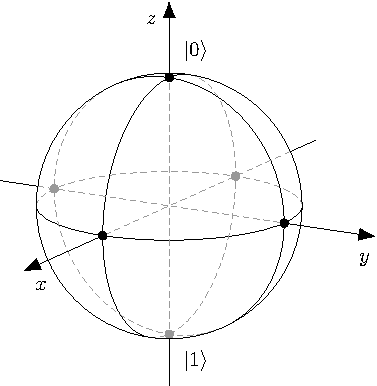
\includegraphics[scale=1]{\exerpath/Figures/sphere_bloch_void.pdf}
%     % \caption{Positions d'états quantiques notables sur la sphère de Bloch. }
%     % \label{fig:sphere_bloch_etats_speciaux}
% \end{figure}